%%%%%%%%%%%%%%%%%%%%%%%%%%%%%%%%%%%%%%%%%%%%%%%%%%%%%%%%%%%%%%%%%%%%%%%%%%%
%% This file is part of the book
%%
%% Algorithmic Graph Theory
%% http://code.google.com/p/graph-theory-algorithms-book/
%%
%% Copyright (C) 2009, 2010, 2011 Minh Van Nguyen <nguyenminh2@gmail.com>
%%
%% See the file COPYING for copying conditions.
%%%%%%%%%%%%%%%%%%%%%%%%%%%%%%%%%%%%%%%%%%%%%%%%%%%%%%%%%%%%%%%%%%%%%%%%%%%

\documentclass{article}

\usepackage{tikz}
\usetikzlibrary{external}
\usetikzlibrary{shapes}
\tikzexternalize{marriage-ties-Renaissance}

\begin{document}

\begin{figure}
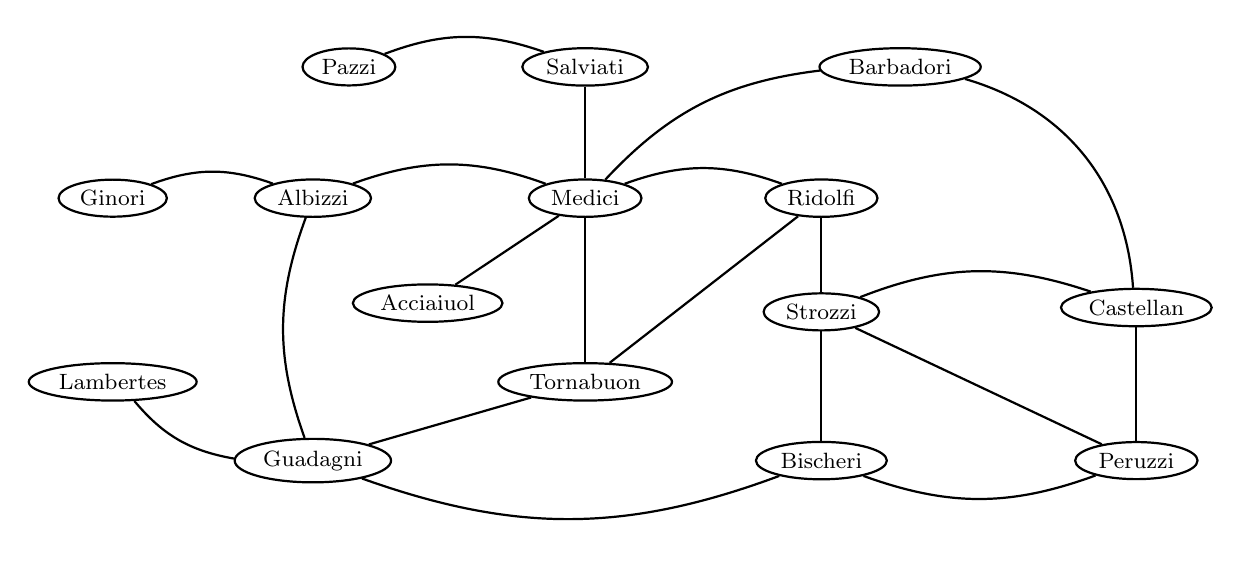
\begin{tikzpicture}
[lineDecorate/.style={-,thick},%
  nodeDecorate/.style={shape=ellipse,inner sep=2pt,draw,thick}]
%% nodes or vertices
\foreach \nodename/\x/\y in {
  Acciaiuol/4/1, Albizzi/2.542/2.333, Barbadori/10/4,
  Bischeri/9/-1, Castellan/13/0.944, Ginori/0/2.333,
  Guadagni/2.542/-1, Lambertes/0/0, Medici/6/2.333,
  Pazzi/3/4, Peruzzi/13/-1, Ridolfi/9/2.333,
  Salviati/6/4, Strozzi/9/0.889, Tornabuon/6/0}
{
  \node (\nodename) at (\x,\y) [nodeDecorate] {\footnotesize\nodename};
}
%% edges or lines
\path
\foreach \startnode/\endnode/\bend/\angle in {
  Acciaiuol/Medici/bend left/0, Albizzi/Guadagni/bend right/20,
  Albizzi/Medici/bend left/20, Barbadori/Castellan/bend left/35,
  Bischeri/Peruzzi/bend right/20, Bischeri/Strozzi/bend left/0,
  Ginori/Albizzi/bend left/20, Guadagni/Bischeri/bend right/20,
  Guadagni/Tornabuon/bend left/0, Lambertes/Guadagni/bend right/20,
  Medici/Barbadori/bend left/20, Medici/Ridolfi/bend left/20,
  Pazzi/Salviati/bend left/20, Peruzzi/Castellan/bend left/0,
  Ridolfi/Strozzi/bend left/0, Salviati/Medici/bend left/0,
  Strozzi/Castellan/bend left/20, Strozzi/Peruzzi/bend left/0,
  Tornabuon/Medici/bend left/0, Tornabuon/Ridolfi/bend left/0}
{
  (\startnode) edge[lineDecorate,\bend=\angle] node {} (\endnode)
};
\end{tikzpicture}
\end{figure}

\end{document}
